\documentclass[aspectratio=169, table]{beamer}

\usepackage{colortbl}
\usepackage{xcolor}
\usepackage{listings}
\usepackage{pgfplots}
\usepgfplotslibrary{polar}
\usepackage{tikz}
\usetikzlibrary{shapes.geometric,
	positioning, shapes, shapes.multipart, backgrounds, arrows.meta, calc, fit, trees}

\usetheme{Pradita}
\arrayrulecolor{black}
\setlength{\arrayrulewidth}{0.2pt}

\lstdefinelanguage{yaml}{
  keywords={true,false,null,yes,no},
  keywordstyle=\color{blue}\bfseries,
  sensitive=false,
  comment=[l]{\#},
  commentstyle=\color{gray}\ttfamily,
  stringstyle=\color{purple}\ttfamily,
  basicstyle=\ttfamily\scriptsize,
  numbers=left,
  numberstyle=\tiny\color{gray},
  breaklines=true,
  frame=lines,
  backgroundcolor=\color{lightgray!10},
  showstringspaces=false
}

\lstdefinelanguage{bash} {
	keywords={},
	basicstyle=\ttfamily\scriptsize,
	keywordstyle=\color{blue}\bfseries,
	ndkeywords={iex},
	ndkeywordstyle=\color{purple}\bfseries,
	sensitive=true,
	commentstyle=\color{gray},
	stringstyle=\color{red},
	numbers=left,
	numberstyle=\tiny\color{gray},
	breaklines=true,
	frame=lines,
	backgroundcolor=\color{lightgray!10},
	tabsize=2,
	comment=[l]{\#},
	morecomment=[s]{/*}{*/},
	commentstyle=\color{gray}\ttfamily,
	stringstyle=\color{purple}\ttfamily,
	showstringspaces=false,
	captionpos=b
}

\lstdefinelanguage{emfatic}{
  keywords={package,enum,class,abstract,attr,ref,val,extends},
  keywordstyle=\color{blue}\bfseries,
  sensitive=true,
  comment=[l]{//},
  commentstyle=\color{gray}\ttfamily,
  basicstyle=\ttfamily\scriptsize,
  numbers=left,
  numberstyle=\tiny\color{gray},
  breaklines=true,
  frame=lines,
  backgroundcolor=\color{lightgray!10},
  showstringspaces=false
}

\lstdefinelanguage{mediaflow}{
  keywords={graph,resource,scaler,transcoder,port,edge,from,to,backend,command,replicas,width,height,mediaType,uri,external},
  keywordstyle=\color{blue}\bfseries,
  sensitive=true,
  comment=[l]{\#},
  commentstyle=\color{gray}\ttfamily,
  stringstyle=\color{purple}\ttfamily,
  basicstyle=\ttfamily\scriptsize,
  numbers=left,
  numberstyle=\tiny\color{gray},
  breaklines=true,
  frame=lines,
  backgroundcolor=\color{lightgray!10},
  showstringspaces=false
}

\lstdefinestyle{JavaStyle}{
  language=Java,
  basicstyle=\ttfamily\scriptsize,
  keywordstyle=\color{blue}\bfseries,
  commentstyle=\color{gray}\ttfamily,
  stringstyle=\color{purple}\ttfamily,
  numbers=left,
  numberstyle=\tiny\color{gray},
  breaklines=true,
  frame=lines,
  backgroundcolor=\color{lightgray!10},
  showstringspaces=false
}

\subtitle{IT30213 - Advanced Software Engineering \& DevOps}
\title{\Huge Textual Domain-\vspace{8pt}\\
	Specific Language}
\author{\textbf{Alfa Yohannis}}

\begin{document}

\frame{\titlepage}

\begin{frame}[fragile]
	\frametitle{Contents}
	\vspace{20pt}
	\begin{columns}[t]
		\column{0.5\textwidth}
		\tableofcontents[sections={1-5}]

		\column{0.5\textwidth}
		\tableofcontents[sections={6-9}]
	\end{columns}
\end{frame}

\begin{frame}{\hfill}
	\centering
	\Huge{\textbf{How do we avoid brittle manual code for complex media 
  large pipeline systems?}}
\end{frame}

\section{Tujuan Pembelajaran}
\begin{frame}{\hfill}
	\centering
	\Huge{\textbf{Tujuan Pembelajaran}}
\end{frame}

\begin{frame}{Tujuan Pembelajaran}
\vspace{6pt}
Setelah sesi ini, mahasiswa diharapkan mampu:
\begin{enumerate}
  \item Menjelaskan keterbatasan koding pipeline media secara manual dan alasan perlunya DSL.
  \item Menerapkan metodologi umum pengembangan DSL dari domain problem sampai transformasi artefak.
  \item Menganalisis trade-off ANTLR, Xtext, dan Langium untuk memilih pendekatan yang sesuai konteks.
\end{enumerate}
\end{frame}

\section{Pendahuluan}
\begin{frame}{\hfill}
	\centering
	\Huge{\textbf{Pendahuluan}}
\end{frame}

\begin{frame}{Masalah Saat Pipeline Dikoding Manual}
\vspace{6pt}
\begin{itemize}
  \item Definisi alur tersebar di banyak skrip/perintah teknis.
  \item Relasi koneksi antar komponen rentan salah referensi.
  \item Parameter transformasi mudah inkonsisten antar environment.
  \item Perubahan requirement memicu edit manual berulang.
  \item Error sering baru terlihat saat integrasi/runtime.
\end{itemize}
\end{frame}

\begin{frame}{Mengapa Perlu DSL?}
\vspace{6pt}
\begin{itemize}
  \item DSL menaikkan abstraksi dari skrip teknis ke model domain.
  \item Struktur pipeline dinyatakan deklaratif sebagai graf.
  \item Validasi dapat dilakukan sebelum eksekusi.
  \item Model dapat ditransform ke artefak target (XMI/JSON/dll).
  \item Evolusi kebutuhan menjadi lebih terkontrol.
\end{itemize}
\end{frame}

\section{Deskripsi Masalah Domain}
\begin{frame}{\hfill}
	\centering
	\Huge{\textbf{Deskripsi Masalah Domain}}
\end{frame}

\begin{frame}{Konteks Domain MediaFlow}
\vspace{6pt}
\begin{itemize}
  \item \textbf{Domain:} orkestrasi pemrosesan media end-to-end.
  \item \textbf{Skenario umum:} satu input master menjadi banyak output.
  \item Pipeline direpresentasikan sebagai graf terarah.
\end{itemize}

\vspace{4pt}
\begin{columns}[T]
\column{0.5\textwidth}
\textbf{Elemen inti}
\begin{itemize}
  \item \textbf{\texttt{Resource}:} sumber/tujuan media
  \item \textbf{\texttt{Scaler}:} transformasi resolusi
  \item \textbf{\texttt{Transcoder}:} transformasi codec/container
\end{itemize}

\column{0.5\textwidth}
\textbf{Relasi}
\begin{itemize}
  \item \textbf{\texttt{Port}:} titik masuk/keluar data
  \item \textbf{\texttt{Edge}:} koneksi antar-port
  \item \textbf{\texttt{Graph}:} kumpulan node + edge
\end{itemize}
\end{columns}
\end{frame}

\begin{frame}{Visual Pipeline Bercabang (Domain Problem)}
\vspace{6pt}
\centering
\scalebox{0.69}{
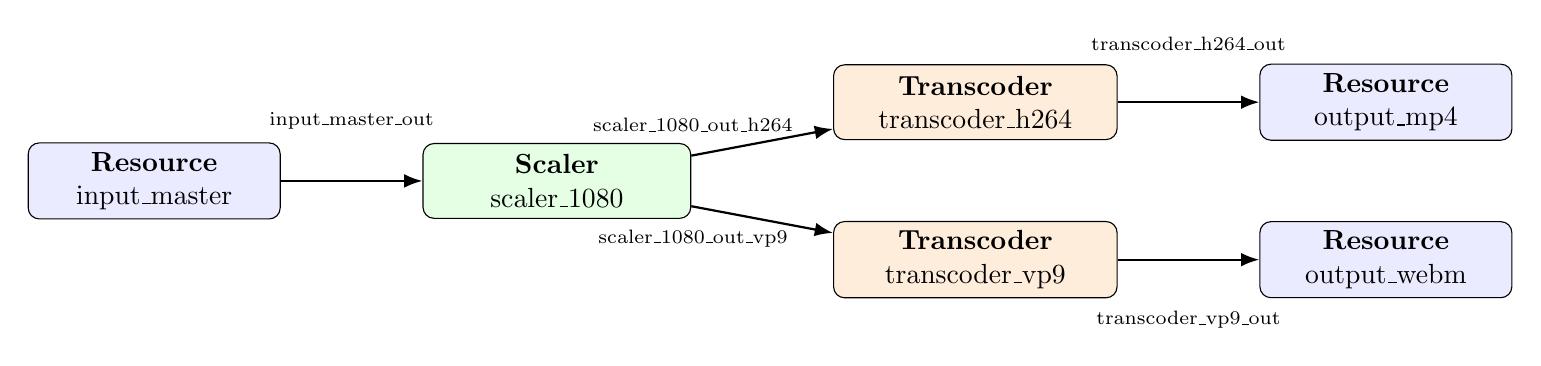
\begin{tikzpicture}[
  node distance=18mm and 18mm,
  >=Latex,
  res/.style={draw, rounded corners, minimum width=3.2cm, minimum height=0.95cm, align=center, fill=blue!8},
  scl/.style={draw, rounded corners, minimum width=3.4cm, minimum height=0.95cm, align=center, fill=green!10},
  trn/.style={draw, rounded corners, minimum width=3.6cm, minimum height=0.95cm, align=center, fill=orange!14},
  arr/.style={->, thick}
]
  \node[res] (input) {\textbf{Resource}\\input\_master};
  \node[scl, right=of input] (scaler1080) {\textbf{Scaler}\\scaler\_1080};
  \node[trn, right=of scaler1080, yshift=10mm] (h264) {\textbf{Transcoder}\\transcoder\_h264};
  \node[trn, right=of scaler1080, yshift=-10mm] (vp9) {\textbf{Transcoder}\\transcoder\_vp9};
  \node[res, right=of h264] (outmp4) {\textbf{Resource}\\output\_mp4};
  \node[res, right=of vp9] (outwebm) {\textbf{Resource}\\output\_webm};

  \draw[arr] (input) -- node[above, font=\scriptsize, yshift=15pt]{input\_master\_out} (scaler1080);
  \draw[arr] (scaler1080) -- node[above, font=\scriptsize, xshift=-25pt]{scaler\_1080\_out\_h264} (h264);
  \draw[arr] (scaler1080) -- node[below, font=\scriptsize, xshift=-25pt]{scaler\_1080\_out\_vp9} (vp9);
  \draw[arr] (h264) -- node[above, font=\scriptsize, yshift=15pt]{transcoder\_h264\_out} (outmp4);
  \draw[arr] (vp9) -- node[below, font=\scriptsize, yshift=-15pt]{transcoder\_vp9\_out} (outwebm);
\end{tikzpicture}
}
\vspace{6pt}
\small
Topologi bercabang seperti ini sulit dipelihara jika ditulis manual tanpa model domain formal.
\end{frame}

\begin{frame}[fragile]{Target DSL Bersama (Semua Solusi)}
\vspace{4pt}
\begin{lstlisting}[language=mediaflow]
graph demo {
  resource inputVideo [mediaType=VIDEO] uri="file:///home/alfa/videos/input.mp4" external=true {
    port inputOut OUT
  }

  scaler resize720 backend=FFMPEG command="ffmpeg -i input.mp4 -vf scale=1280:720 scaled.mp4" replicas=1 width=1280 height=720 {
    port resizeIn IN
    port resizeOut OUT
  }

  edge e1 from inputOut to resizeIn
}
\end{lstlisting}
\vspace{2pt}
\small
Model ini menjadi target parsing yang sama untuk ANTLR, Xtext, dan Langium.
\end{frame}

\begin{frame}{Masalah Utama dan Kebutuhan Pemodelan}
\vspace{4pt}
\begin{columns}[T]
\column{0.5\textwidth}
\textbf{Masalah Utama}
\begin{itemize}
  \item Topologi makin kompleks
  \item Konfigurasi tidak konsisten
  \item Referensi koneksi rawan salah
  \item Perubahan requirement mahal
  \item Sulit telusur desain vs implementasi
\end{itemize}

\column{0.5\textwidth}
\textbf{Kebutuhan Pemodelan}
\begin{itemize}
  \item Representasi deklaratif berbasis graf
  \item Abstract model stabil
  \item Validasi struktural + domain
  \item Linking referensi deterministik
  \item Transformasi ke artefak turunan
\end{itemize}
\end{columns}
\end{frame}

\section{Metodologi Umum Pemodelan}
\begin{frame}{\hfill}
	\centering
	\Huge{\textbf{Metodologi Umum Pemodelan}}
\end{frame}

\begin{frame}{Peta Metodologi Umum (8 Tahap)}
\vspace{4pt}
\begin{enumerate}
  \item Perumusan batas domain
  \item Identifikasi konsep inti dan relasi
  \item Perancangan abstract model
  \item Definisi aturan semantik dan validasi
  \item Perancangan concrete syntax
  \item Parsing, linking, dan resolusi referensi
  \item Transformasi model dan artefak
  \item Strategi pengujian dan iterasi
\end{enumerate}
\end{frame}

\begin{frame}{Langkah 1-2: Domain dan Konsep Inti}
\scriptsize
\begin{itemize}
  \item \textbf{Langkah 1: Perumusan Batas Domain}
  \begin{itemize}
    \item \textbf{Input:} problem statement, tujuan stakeholder, batasan teknis.
    \item \textbf{Output:} domain scope statement (in-scope/out-of-scope).
    \item \textbf{Contoh:} In-scope memodelkan \texttt{Resource/Scaler/Transcoder}. \texttt{Resource} berarti sumber/tujuan media (misalnya file \texttt{.mp4}); out-of-scope tidak mencakup autoscaling cluster.
  \end{itemize}
  \item \textbf{Langkah 2: Identifikasi Konsep Inti dan Relasi}
  \begin{itemize}
    \item \textbf{Input:} scope domain dan skenario alur.
    \item \textbf{Output:} daftar konsep + glosarium + peta relasi.
    \item \textbf{Contoh:} \texttt{input\_master} sebagai \texttt{Resource}, \texttt{scaler\_1080} sebagai \texttt{Scaler}, dan \texttt{edge\_scaler\_to\_h264} sebagai \texttt{Edge}.
  \end{itemize}
\end{itemize}
\end{frame}

\begin{frame}{Langkah 3-4: Abstract Model dan Validasi}
\scriptsize
\begin{itemize}
  \item \textbf{Langkah 3: Perancangan Abstract Model}
  \begin{itemize}
    \item \textbf{Input:} konsep inti dan relasi domain.
    \item \textbf{Output:} metamodel/AST dengan kardinalitas dan referensi.
    \item \textbf{Contoh:} \texttt{Graph.nodes[*]} berarti daftar node 0..* (misalnya \texttt{input\_master}, \texttt{scaler\_1080}, \texttt{transcoder\_h264}); \texttt{Edge.source/target} mereferensikan \texttt{Port}.
  \end{itemize}
  \item \textbf{Langkah 4: Definisi Aturan Semantik dan Validasi}
  \begin{itemize}
    \item \textbf{Input:} abstract model + aturan domain.
    \item \textbf{Output:} katalog aturan validasi dan severity.
    \item \textbf{Contoh:} \texttt{OUT->IN} valid, sedangkan \texttt{IN->IN} ditolak.
  \end{itemize}
\end{itemize}
\end{frame}

\begin{frame}{Langkah 5-6: Concrete Syntax dan Linking}
\scriptsize
\begin{itemize}
  \item \textbf{Langkah 5: Perancangan Concrete Syntax}
  \begin{itemize}
    \item \textbf{Input:} abstract model + aturan validasi.
    \item \textbf{Output:} grammar awal + konvensi penulisan model.
    \item \textbf{Contoh:} \texttt{resource input1 ...} dan \texttt{edge e1 from inputOut to resizeIn}.
  \end{itemize}
  \item \textbf{Langkah 6: Parsing, Linking, Resolusi Referensi}
  \begin{itemize}
    \item \textbf{Input:} grammar + aturan scope + model contoh.
    \item \textbf{Output:} parser aktif + hasil linking + diagnostik.
    \item \textbf{Contoh:} token \texttt{inputOut} dipetakan ke objek \texttt{Port}; jika tidak ada maka muncul error linking.
  \end{itemize}
\end{itemize}
\end{frame}

\begin{frame}{Langkah 7-8: Transformasi dan Iterasi}
\scriptsize
\begin{itemize}
  \item \textbf{Langkah 7: Transformasi Model dan Artefak}
  \begin{itemize}
    \item \textbf{Input:} model valid + spesifikasi format target.
    \item \textbf{Output:} artefak turunan (XMI/JSON/dll) + prosedur generate repeatable.
    \item \textbf{Contoh:} \texttt{test.mediaflow} $\rightarrow$ \texttt{output/test.xmi} dan \texttt{output/test.json}.
  \end{itemize}
  \item \textbf{Langkah 8: Strategi Pengujian dan Iterasi}
  \begin{itemize}
    \item \textbf{Input:} parser/linking/validator/generator + korpus uji.
    \item \textbf{Output:} hasil uji, daftar perbaikan, baseline bahasa berversi.
    \item \textbf{Contoh:} test edge ke port yang tidak ada harus gagal, lalu grammar/scope diperbaiki dan versi dinaikkan.
  \end{itemize}
\end{itemize}
\end{frame}

\section{Implementasi Detail dengan ANTLR}
\begin{frame}{\hfill}
	\centering
	\Huge{\textbf{Implementasi Detail dengan ANTLR}}
\end{frame}

\begin{frame}{Arsitektur ANTLR}
\vspace{4pt}
\begin{enumerate}
  \item \textbf{Grammar DSL \texttt{MediaFlow.g4}:} mendefinisikan token dan rule inti (\texttt{graph}, \texttt{node}, \texttt{edge}).
  \item \textbf{Artefak generasi:} lexer, parser, dan visitor untuk membentuk parse tree dari dokumen DSL.
  \item \textbf{Kelas AST domain \texttt{Graph/Node/Port/Edge}:} representasi semantik terpisah dari parse tree ANTLR.
  \item \textbf{\texttt{AstBuilder}:} memetakan parse tree ke AST, termasuk registrasi simbol sebelum linking.
  \item \textbf{Entry point:} membaca file input, menjalankan parser, lalu membangun model AST siap validasi.
\end{enumerate}
\vspace{6pt}
\small
Kekuatan utama ANTLR adalah kontrol implementasi yang sangat detail. Tantangan utamanya, seluruh linking simbol dan validasi domain perlu dirancang manual oleh developer.
\end{frame}

\begin{frame}[fragile]{Potongan Grammar ANTLR (Struktur Utama)}
\vspace{4pt}
\begin{columns}[T,onlytextwidth]
\column{0.52\textwidth}
\begin{lstlisting}[language=bash]
model : graph EOF ;

graph
  : 'graph' name=ID '{'
      node*
      edge*
    '}'
  ;

edge
  : 'edge' name=ID
    'from' source=ID
    'to' target=ID
  ;

ID : [a-zA-Z_][a-zA-Z_0-9]* ;
\end{lstlisting}
\column{0.44\textwidth}
\small
\textbf{Penjelasan}
\begin{itemize}
  \item \texttt{model} adalah entry rule; \texttt{EOF} memastikan input habis diparse.
  \item \textbf{\texttt{graph} mendefinisikan struktur dokumen:} deklarasi node diikuti edge.
  \item \texttt{edge} menghubungkan dua identifier port melalui \texttt{from}/\texttt{to}.
  \item Rule lexer \texttt{ID} menentukan pola nama simbol untuk elemen domain.
\end{itemize}
\end{columns}
\end{frame}

\begin{frame}[fragile]{Linking Manual pada AstBuilder}
\vspace{10pt}
\begin{lstlisting}[style=JavaStyle, basicstyle=\ttfamily\scriptsize]
private void resolveEdges() {
    for (Edge e : unresolvedEdges) {
        e.source = portIndex.get(e.sourceName);
        e.target = portIndex.get(e.targetName);
        if (e.source == null) throw new RuntimeException("Unknown source");
        if (e.target == null) throw new RuntimeException("Unknown target");
    }
}
\end{lstlisting}
\vspace{2pt}
\small
\begin{itemize}
  \item \textbf{Proses dibuat dua tahap:} semua \texttt{Port} didaftarkan dulu ke \texttt{portIndex}, lalu setiap \texttt{Edge} diselesaikan pada \texttt{resolveEdges()}.
  \item \texttt{sourceName}/\texttt{targetName} awalnya masih string; method ini mengubahnya menjadi referensi objek \texttt{Port} yang valid.
  \item Jika port tidak ditemukan, parser berhenti dengan error \texttt{Unknown source/target} agar model salah tidak lanjut ke tahap transformasi.
\end{itemize}
\end{frame}

\section{Implementasi Detail dengan Xtext}
\begin{frame}{\hfill}
	\centering
	\Huge{\textbf{Implementasi Detail dengan Xtext}}
\end{frame}

\begin{frame}{Arsitektur Xtext}
\vspace{4pt}
\begin{enumerate}
  \item \textbf{Grammar Xtext \texttt{MediaFlow.xtext}:} mendefinisikan bentuk concrete syntax DSL.
  \item \textbf{Binding metamodel EMF (\texttt{returns mediaflow::...}):} rule grammar langsung dipetakan ke Ecore.
  \item \textbf{Runtime services bawaan:} parser, linker, serializer, dan diagnostik model.
  \item \textbf{Kustomisasi domain:} \texttt{ScopeProvider} dan \texttt{Validator} untuk aturan semantik.
  \item \textbf{Tooling modules:} \texttt{runtime/UI/IDE/web} untuk dukungan editor yang lebih lengkap.
\end{enumerate}
\vspace{4pt}
\small
Pendekatan ini cocok saat tim butuh produktivitas model-driven dan integrasi kuat dengan ekosistem EMF/Eclipse.
\end{frame}

\begin{frame}[fragile]{Grammar Xtext: Binding + Cross-Reference}
\vspace{4pt}
\begin{columns}[T,onlytextwidth]
\column{0.52\textwidth}
\begin{lstlisting}[language=bash]
Model returns mediaflow::Graph:
    Graph
;

Graph returns mediaflow::Graph:
    'graph' name=ID '{'
        nodes+=Node*
        edges+=Edge*
    '}'
;

Edge returns mediaflow::Edge:
    'edge' name=ID
    'from' source=[mediaflow::Port|ID]
    'to' target=[mediaflow::Port|ID]
;
\end{lstlisting}
\column{0.44\textwidth}
\small
\textbf{Penjelasan}
\begin{itemize}
  \item \textbf{\texttt{returns mediaflow::...}:} mengikat rule grammar langsung ke metamodel EMF.
  \item \texttt{nodes+=} dan \texttt{edges+=} menambahkan koleksi elemen ke objek \texttt{Graph}.
  \item \textbf{Notasi \texttt{[mediaflow::Port|ID]}:} menyatakan cross-reference berbasis simbol.
  \item Scope provider menentukan kandidat referensi agar \texttt{source}/\texttt{target} tidak ambigu.
\end{itemize}
\end{columns}
\end{frame}

\begin{frame}{Scope, Validator, dan Build Xtext}
\vspace{4pt}
\begin{itemize}
  \item \textbf{Scope Provider}: membatasi kandidat \texttt{Port} pada \texttt{Graph} yang sama.
  \item \textbf{Validator}: tempat aturan domain (\texttt{@Check}) seperti arah port dan konsistensi koneksi.
  \item \textbf{Build}: \texttt{mvn -f mediaflow.xtext.parent/pom.xml clean verify}
\end{itemize}
\vspace{6pt}
\small
Kekuatan Xtext: ekosistem model-driven yang lengkap. Tantangan: setup multi-modul Tycho lebih kompleks.
\end{frame}

\section{Implementasi Detail dengan Langium}
\begin{frame}{\hfill}
	\centering
	\Huge{\textbf{Implementasi Detail dengan Langium}}
\end{frame}

\begin{frame}{Arsitektur Langium}
\vspace{4pt}
\begin{enumerate}
  \item \textbf{Grammar Langium \texttt{media-flow.langium}:} mendefinisikan struktur bahasa dan referensi.
  \item \textbf{Generated AST/services (TypeScript):} tipe AST dan layanan language server dihasilkan otomatis.
  \item \textbf{Kustomisasi \texttt{scope} + \texttt{validator}:} memastikan resolusi simbol dan aturan domain konsisten.
  \item \textbf{CLI generator (\texttt{packages/cli}):} menurunkan model ke artefak output (misalnya ELK JSON).
  \item \textbf{VS Code extension (\texttt{packages/extension}):} menyediakan pengalaman authoring DSL yang modern.
\end{enumerate}
\vspace{6pt}
\small
Fokus utama Langium adalah tooling modern di stack Node.js/TypeScript dengan siklus iterasi cepat dari grammar ke editor dan generator.
\end{frame}

\begin{frame}[fragile]{Grammar dan Referensi pada Langium}
\vspace{4pt}
\begin{columns}[T,onlytextwidth]
\column{0.52\textwidth}
\begin{lstlisting}[language=bash]
entry Model:
    elements+=Element*;

Edge:
    'edge' name=ID
    'from' source=[Port:QualifiedPortName]
    'to' target=[Port:QualifiedPortName]
;

QualifiedPortName returns string:
    ID ('.' ID)?
;
\end{lstlisting}
\column{0.44\textwidth}
\small
\textbf{Penjelasan}
\begin{itemize}
  \item \texttt{entry Model} menjadi titik masuk parser untuk seluruh dokumen DSL.
  \item \textbf{Rule \texttt{Edge} menyimpan dua referensi simbol:} \texttt{source} dan \texttt{target}.
  \item \texttt{QualifiedPortName} mendukung nama sederhana dan format \texttt{node.port}.
  \item Nama berkualifikasi membantu mencegah benturan simbol saat model membesar.
\end{itemize}
\end{columns}
\end{frame}

\begin{frame}[fragile]{Generator CLI Langium}
\vspace{4pt}
\begin{lstlisting}[language=bash]
cd mediaflow-langium/mediaflow
npm run langium:generate
npm run build
node ./packages/cli/bin/cli.js generate ./input/test.mediaflow ./output/test.json
\end{lstlisting}
\vspace{2pt}
\small
Output utama studi kasus: ELK JSON untuk visualisasi/layout graph. Urutan command menegaskan ketergantungan proses: generate artefak grammar, build workspace, lalu eksekusi CLI agar parser dan tipe AST tetap sinkron.
\end{frame}

\begin{frame}{Strategi Pengujian Umum (Semua Solusi)}
\vspace{4pt}
\begin{itemize}
  \item \textbf{Uji parsing}: model valid/invalid.
  \item \textbf{Uji linking}: referensi port benar, termasuk kasus \textit{unknown} atau \textit{duplicate} port.
  \item \textbf{Uji validasi semantik}: aturan domain seperti arah koneksi \texttt{OUT->IN}.
  \item \textbf{Uji generator/output}: artefak target konsisten untuk model input yang sama.
\end{itemize}
\vspace{4pt}
\textbf{Set minimum test case}
\begin{itemize}
  \item 1 model valid (\textit{happy path})
  \item 1 model dengan referensi port salah
  \item 1 model yang melanggar aturan domain
\end{itemize}
\end{frame}

\section{Perbandingan ANTLR vs Xtext vs Langium}
\begin{frame}{\hfill}
	\centering
	\Huge{\textbf{Perbandingan ANTLR vs Xtext vs Langium}}
\end{frame}

\begin{frame}{Perbandingan Aspek Teknis}
\scriptsize
\arrayrulecolor{black}
\begin{tabular}{|p{0.11\textwidth}|p{0.25\textwidth}|p{0.25\textwidth}|p{0.25\textwidth}|}
\hline
\textbf{Aspek} & \textbf{ANTLR} & \textbf{Xtext} & \textbf{Langium} \\
\hline
Fokus utama & Kontrol parser rendah-level & DSL berbasis EMF lengkap & DSL modern TypeScript \\
\hline
Representasi model & AST manual (visitor) & Bind ke Ecore & AST generated \\
\hline
Linking & Manual (symbol table) & Cross-ref + scope & Ref-resolution + scope \\
\hline
Validasi domain & Manual penuh & \texttt{@Check} validator & Validation checks service \\
\hline
Runtime utama & Java/JVM & Java + Eclipse/EMF & Node.js/TypeScript \\
\hline
Implikasi praktis & Fleksibel dan transparan, tetapi banyak komponen manual. & Produktif untuk ekosistem model-driven enterprise. & Cepat diadopsi tim web dengan tooling VS Code modern. \\
\hline
\end{tabular}
\end{frame}

\begin{frame}{Perbandingan Tooling dan Produktivitas}
\scriptsize
\arrayrulecolor{black}
\begin{tabular}{|p{0.11\textwidth}|p{0.25\textwidth}|p{0.25\textwidth}|p{0.25\textwidth}|}
\hline
\textbf{Aspek} & \textbf{ANTLR} & \textbf{Xtext} & \textbf{Langium} \\
\hline
Kurva belajar & Menengah & Menengah-tinggi & Rendah-menengah (tim JS) \\
\hline
Editor support & Bangun sendiri/terpisah & Kuat di Eclipse & Kuat di VS Code \\
\hline
Build \& CI & Relatif sederhana & Tycho multi-modul lebih kompleks & Ringan (npm workspace) \\
\hline
Kesesuaian tim & Tim compiler/parser & Tim model-driven EMF & Tim web/platform JS \\
\hline
Implikasi tim & Kontrol tinggi dengan effort implementasi lebih besar. & Investasi awal tinggi, maintainability kuat di proyek besar. & Produktivitas cepat dengan workflow Node.js yang familiar. \\
\hline
\end{tabular}
\end{frame}

\begin{frame}{Panduan Pemilihan Pendekatan}
\vspace{4pt}
\begin{itemize}
  \item \textbf{Pilih ANTLR}: jika butuh kontrol penuh grammar + linking manual.
  \item \textbf{Pilih Xtext}: jika butuh integrasi kuat dengan EMF/Ecore dan tooling Eclipse.
  \item \textbf{Pilih Langium}: jika target utama VS Code, TypeScript, dan iterasi cepat.
\end{itemize}
\vspace{8pt}
\textbf{Urutan belajar yang direkomendasikan}
\begin{enumerate}
  \item ANTLR (fondasi parser/linking)
  \item Xtext (otomatisasi model-driven)
  \item Langium (tooling modern)
\end{enumerate}
\end{frame}

\section{Ringkasan}
\begin{frame}{\hfill}
	\centering
	\Huge{\textbf{Ringkasan}}
\end{frame}

\begin{frame}{Kesimpulan Sesi}
\small
\begin{itemize}
  \item Koding pipeline manual tidak skalabel untuk topologi dan variasi konfigurasi kompleks.
  \item Target DSL MediaFlow dapat dipakai konsisten pada ANTLR, Xtext, dan Langium.
  \item Metodologi 8 tahap memberi alur sistematis dari domain problem hingga artefak turunan.
  \item Pengujian inti (parsing, linking, validasi, generator) berlaku sama untuk semua solusi.
  \item \textbf{Pemilihan tool tetap berbasis trade-off:} kontrol (ANTLR), ekosistem EMF (Xtext), atau tooling modern TS/VS Code (Langium).
\end{itemize}
\end{frame}

\end{document}
